\documentclass[10pt,letterpaper]{article}

\usepackage[letterpaper,margin=0.70in,headheight=22pt,headsep=16pt,footskip=24pt]{geometry}
\usepackage[T1]{fontenc}
\usepackage[utf8]{inputenc}
\usepackage{lmodern}
\usepackage{microtype}
\usepackage{xcolor}
\usepackage{graphicx}
\usepackage{booktabs}
\usepackage{array}
\usepackage{tabularx}
\usepackage{longtable}
\usepackage{amsmath,amssymb}
\usepackage{tikz}
\usetikzlibrary{arrows.meta,positioning,calc,shapes.geometric,decorations.pathreplacing,fit}
\usepackage{enumitem}
\usepackage{fancyhdr}
\usepackage{titlesec}
\usepackage{caption}
\usepackage{listings}
\usepackage{xurl}
\usepackage[hidelinks]{hyperref}
\usepackage{lastpage}
\usepackage{float}
\usepackage{placeins}

% WVURAIL house palette: shared neutrals, per-project accent.
% PilotProxy uses FStatRed (A00000); datatrawl uses TrawlAmber.
\definecolor{TrawlAmber}{HTML}{A66A00}
\definecolor{TrawlGray}{HTML}{555555}
\definecolor{TrawlBlue}{HTML}{144E8C}
\definecolor{LightGray}{HTML}{F3F3F3}
\definecolor{MidGray}{HTML}{D9D9D9}
\definecolor{DarkText}{HTML}{1A1A1A}
\definecolor{GoodGreen}{HTML}{2B7A2B}
\definecolor{WarnOrange}{HTML}{A65E00}

\renewcommand{\familydefault}{\sfdefault}
\setlength{\parindent}{0pt}
\setlength{\parskip}{5pt}
\renewcommand{\arraystretch}{1.15}
\sloppy
\setlist[itemize]{leftmargin=1.2em,itemsep=2pt,topsep=2pt}
\setlist[enumerate]{leftmargin=1.4em,itemsep=2pt,topsep=2pt}

\titleformat{\section}{\Large\bfseries\color{DarkText}}{}{0pt}{}[\vspace{-3pt}\color{TrawlAmber}\titlerule]
\titleformat{\subsection}{\large\bfseries\color{DarkText}}{}{0pt}{}
\titleformat{\subsubsection}{\normalsize\bfseries\color{DarkText}}{}{0pt}{}

\newcommand{\code}[1]{\texttt{\detokenize{#1}}}
\newcommand{\apicode}[1]{\texttt{\detokenize{#1}}}
\newcommand{\yes}{\textcolor{GoodGreen}{Yes}}
\newcommand{\no}{\textcolor{TrawlGray}{No}}
\newcolumntype{Y}{>{\raggedright\arraybackslash}X}
\newcolumntype{L}[1]{>{\raggedright\arraybackslash}p{#1}}
\newcolumntype{C}[1]{>{\centering\arraybackslash}p{#1}}
\captionsetup{font=small,labelfont=bf}

\lstdefinestyle{shell}{
  basicstyle=\ttfamily\footnotesize,
  breaklines=true,
  columns=fullflexible,
  frame=single,
  rulecolor=\color{MidGray},
  backgroundcolor=\color{LightGray},
  keepspaces=true,
  showstringspaces=false
}
\lstset{style=shell}

\newcommand{\notebox}[1]{%
  \vspace{4pt}\noindent\fcolorbox{TrawlBlue}{LightGray}{%
  \begin{minipage}{0.965\linewidth}%
  \textbf{Note:} #1%
  \end{minipage}}\vspace{4pt}}

\newcommand{\importantbox}[1]{%
  \vspace{4pt}\noindent\fcolorbox{TrawlAmber}{LightGray}{%
  \begin{minipage}{0.965\linewidth}%
  \textbf{Important:} #1%
  \end{minipage}}\vspace{4pt}}

\newcommand{\field}[1]{\texttt{\detokenize{#1}}}

\pagestyle{fancy}
\fancyhf{}
\fancyhead[L]{\small Datatrawl-DS001}
\fancyhead[C]{\small Storage-Safe Archive Trawling Engine v0.2.0}
\fancyhead[R]{\small Product Specification}
\fancyfoot[L]{\small Datatrawl-DS001 v1.1}
\fancyfoot[C]{\small West Virginia University}
\fancyfoot[R]{\small Page \thepage\ of \pageref{LastPage}}
\renewcommand{\headrulewidth}{0.8pt}
\renewcommand{\headrule}{\hbox to\headwidth{\color{TrawlAmber}\leaders\hrule height \headrulewidth\hfill}}
\renewcommand{\footrulewidth}{0.8pt}
\renewcommand{\footrule}{\hbox to\headwidth{\color{TrawlAmber}\leaders\hrule height \footrulewidth\hfill}}

\title{datatrawl Storage-Safe Archive Trawling Engine v0.2.0\\Product Specification}
\author{West Virginia University}
\date{Datatrawl-DS001 v1.1 \\ July 3, 2026}

\begin{document}
\thispagestyle{fancy}
{\sffamily
\begin{minipage}[t]{0.39\textwidth}
  {\fontsize{24}{26}\selectfont\bfseries\color{TrawlAmber}datatrawl}\par
  {\small Datatrawl-DS001 v1.1, July 3, 2026}
\end{minipage}%
\begin{minipage}[t]{0.61\textwidth}
  \raggedleft
  {\large\bfseries Storage-Safe Archive Trawling Engine}\par
  {\small One file at a time. Resumable. Provenance-carrying.}\par
  {\small West Virginia University Radio Astronomy Instrumentation Lab (RAIL)}
\end{minipage}
}
\vspace{6pt}
{\color{TrawlAmber}\hrule height 1.2pt}
\vspace{8pt}

{\small\color{TrawlGray}This product specification defines the v0.2.0 streaming
engine contract. datatrawl is a downstream run layer: the archive authority
(e.g.\ Datatrail/CADC) remains the source of record for what data exists;
datatrawl fetches, streams, and deletes copies under a fixed storage budget.
Throughput is source-, network-, and analyzer-dependent and should be measured
on the target system.}

\section{Features}
\begin{itemize}
  \item Streams telescope archives \textbf{one file at a time} under a fixed
        local-storage budget: fetch, analyze, delete, checkpoint, repeat.
  \item \textbf{Resumable products}: the analyzer owns its product file,
        re-loads it on restart, and skips already-accumulated units; a
        kill at any point loses at most the work since the last checkpoint.
  \item Four-choice run model --- \field{telescope}, \field{source},
        \field{reader}, \field{analyzer} --- covers the whole configuration
        surface; \code{datatrawl doctor} makes each choice and its
        prerequisites legible before compute time is spent.
  \item \textbf{Pluggable}: sources, readers, analyzers, and telescopes
        register through the \code{datatrawl.plugins} entry-point group or an
        explicit \code{--plugin} module path; external packages (e.g.\
        PilotProxy) ship analyzers without modifying datatrawl.
  \item \textbf{Ordering contract}: analyzers declare
        \field{requires_in_order}; the engine refuses parallel-fetch settings
        that would deliver files out of source order to such analyzers.
  \item Memory-bound inventories: \code{datatrawl survey} writes a named
        inventory directory recording the telescope/source/reader choices, so
        \code{datatrawl scan} needs only the analyzer and the inventory name.
  \item \textbf{Selection}: \field{freq_id}s and/or events, one grammar
        across sources --- \code{614,706}, \code{506-844},
        \code{events:349382977}, or the dict form a \field{plan_runs}
        returns; filters are exact and ANDed, and malformed input fails
        loudly with the grammar named.
  \item \textbf{Archive discovery (recon)}: \code{survey --scopes-only}
        maps scopes and datasets with no event enumeration and no download;
        \code{--match} filters by name, \code{--expand} opens containers one
        level, \code{--name} labels the map, and a scope datatrail fails to
        answer for is reported as an INCOMPLETE map, never as emptiness.
  \item \textbf{Reader-owned archive file shape}: which files one event
        contributes is declared by the reader (\field{survey_files});
        inventory rows are self-describing (each records its file
        \field{name}), so a scan stages exactly what the survey verified.
  \item Atomic product writes (\code{.tmp} then rename), per-invocation
        staging directories (concurrent scans cannot delete each other's
        files), and unit-key provenance embedded in every product.
  \item Pure-Python core (\code{numpy}, \code{h5py}, \code{pyyaml});
        CANFAR/CADC access and GPU acceleration are optional extras.
\end{itemize}

\section{What datatrawl Is and Is Not}
\begin{tabularx}{\linewidth}{L{0.30\linewidth} Y}
\toprule
\textbf{Is} & A run layer that walks an archive inventory, stages one file,
              hands its arrays to a science analyzer, saves a resumable
              product, and deletes the staged copy. \\
\textbf{Is} & A contract between an engine and plugins: lifecycle, ordering,
              resume, and provenance rules that make long unattended runs
              safe. \\
\textbf{Is not} & An archive. Datatrail/CADC remain the authority on what data
              exists and where; datatrawl never mutates archive state. \\
\textbf{Is not} & A scheduler or workflow manager. One \code{scan} is one
              process; independence across products comes from the analyzer's
              \field{plan_runs} split, not from a DAG engine. \\
\textbf{Is not} & A science package. The statistics live in analyzers
              (built-in \code{spectrum}, or external plugins such as the
              PilotProxy detector). \\
\bottomrule
\end{tabularx}

\section{System Overview}
\begin{figure}[H]
\centering
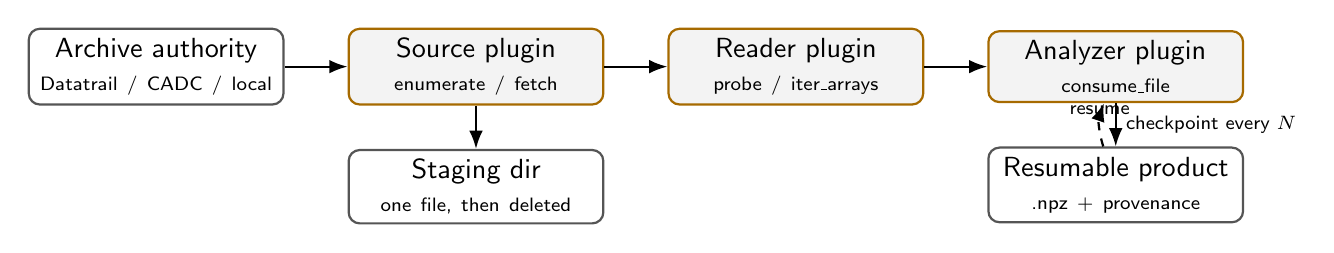
\begin{tikzpicture}[node distance=0.55cm and 0.8cm,>=Latex]
\tikzstyle{blk}=[rectangle,rounded corners,draw=TrawlAmber,thick,fill=LightGray,
                 minimum height=0.85cm,text width=3.0cm,align=center]
\tikzstyle{soft}=[rectangle,rounded corners,draw=TrawlGray,thick,fill=white,
                  minimum height=0.85cm,text width=3.0cm,align=center]
\node[soft] (arch) {Archive authority\\{\scriptsize Datatrail / CADC / local}};
\node[blk,right=of arch] (src) {Source plugin\\{\scriptsize enumerate / fetch}};
\node[blk,right=of src] (rdr) {Reader plugin\\{\scriptsize probe / iter\_arrays}};
\node[blk,right=of rdr] (ana) {Analyzer plugin\\{\scriptsize consume\_file}};
\node[soft,below=of ana] (prod) {Resumable product\\{\scriptsize .npz + provenance}};
\node[soft,below=of src] (stage) {Staging dir\\{\scriptsize one file, then deleted}};
\draw[->,thick] (arch) -- (src);
\draw[->,thick] (src) -- (rdr);
\draw[->,thick] (rdr) -- (ana);
\draw[->,thick] (ana) -- node[right,font=\scriptsize]{checkpoint every $N$} (prod);
\draw[->,thick] (src) -- (stage);
\draw[->,thick,dashed] (prod) to[bend left=18] node[above,font=\scriptsize]{resume} (ana);
\end{tikzpicture}
\caption{One-pass streaming loop. The engine drives the lifecycle; plugins own
archive access, file decoding, and science.}
\end{figure}

\section{Operating Limits and Contracts}
\begin{tabularx}{\linewidth}{L{0.34\linewidth} L{0.22\linewidth} Y}
\toprule
\textbf{Parameter} & \textbf{Value} & \textbf{Contract} \\
\midrule
Staged files on disk & 1 (default) & \code{--max-staged-files} raises the
prefetch depth; refused when the analyzer sets \field{requires_in_order}. \\
Download workers & 1 (default) & \code{--download-workers} parallelizes fetch
only; all accumulator writes stay on the engine's main thread (no analyzer
locking). Refused for in-order analyzers. \\
Checkpoint interval & 50 files & \code{--checkpoint-every}; each checkpoint is
an atomic \code{save()} of the full product. \\
Delivery order & Source order & Guaranteed at the defaults; completion order
otherwise. In-order analyzers can only run at the defaults. \\
Staging directory & Per invocation & Unique path per scan; concurrent scans
cannot delete each other's staged files. \\
Product write & Atomic & \code{<product>.tmp} then rename; a kill never leaves
a partial product. \\
Resume gate & Strict & \field{resume()} must raise on an existing but
incompatible product; two configurations can never mix into one file. \\
Inventory memory & Bounded & Inventory records stream from disk; the engine
never holds the full archive listing in memory. \\
\bottomrule
\end{tabularx}

\section{Command Surface}
\begin{tabularx}{\linewidth}{L{0.28\linewidth} Y}
\toprule
\textbf{Command} & \textbf{Function} \\
\midrule
\code{datatrawl list} & Everything available at a glance; subcommands
\code{telescopes}, \code{readers}, \code{analyzers}, \code{sources}. \\
\code{datatrawl doctor} & Startup checklist and ready-to-go combinations; with
\code{--telescope/--source/--reader/--analyzer}, the checklist for one chosen
combination. \\
\code{datatrawl explore} & Report what data is available for a source
(no download). \\
\code{datatrawl survey} & Walk the archive to build a named inventory
directory; records telescope, source, and reader. With \code{--scopes-only},
recon: map scopes and datasets (\code{--match}, \code{--expand},
\code{--name}) with no event enumeration or download. \\
\code{datatrawl scan} & Run the streaming analyzer over an inventory
(\code{--name}/\code{--inventory}), with \code{--select} interpreted by the
analyzer. \\
\code{datatrawl setup-cupy} & Detect the session image's CUDA version and
install the matching \code{cupy-cudaXXx} wheel. \\
\code{datatrawl --version} & Package and runtime report the same version. \\
\bottomrule
\end{tabularx}

\section{Plugin Interfaces}
\subsection{Analyzer lifecycle}
The analyzer owns its product file: it writes it, re-loads it on resume, and
reports which units it already contains. The engine drives:
\begin{lstlisting}
resume(path, ctx) -> bool     # load an existing, compatible product
processed_keys()  -> set      # Unit.key values already accumulated
begin(ctx, first_meta)        # once, at the first new file
consume_file(arrays, meta)->n # per file; update accumulators
save(path)                    # atomic (re)write, provenance embedded
summary()         -> dict     # one human-readable status line
\end{lstlisting}
Selection hooks \field{resolve_selection} and \field{plan_runs} let an
analyzer interpret \code{--select} and split it into independent, individually
resumable products (e.g.\ one product per \field{freq_id}).

\importantbox{Set \field{requires_in_order = True} for any product that is not
a commutative accumulation (running statistics, CFAR baselines, trailing
windows). The engine then refuses \code{--download-workers}\,/\,%
\code{--max-staged-files} above 1, so an order-dependent analyzer can never
silently consume files in download-completion order.}

\subsection{Source and Reader}
\begin{itemize}
  \item \textbf{Source}: \field{enumerate(ctx)} yields \field{Unit}s;
        \field{fetch(unit, dest)} stages one file; \field{survey(ctx, out)}
        builds an inventory; \field{preflight(ctx)} verifies credentials and
        connectivity before the run starts.
  \item \textbf{Reader}: \field{probe(path)} returns file metadata;
        \field{iter_arrays(path, ctx)} streams decode-ready arrays;
        \field{preflight(ctx)} verifies decode prerequisites. Optionally,
        \field{survey_files(event, common_path, selection, ctx)} declares the
        archive file shape for surveys, and \field{annotate_row} enriches
        verified inventory rows.
\end{itemize}
The Datatrail adapter, re-exported from \code{datatrawl.plugins.sources}, is
the one sanctioned dtcli surface for analyzers and user code;
\field{DATATRAIL.files(scope, dataset)} lists a dataset's files
programmatically (the \code{datatrail ps -s} view) with a contract that
distinguishes a service outage from an empty dataset.

\subsection{Registration}
Plugins register through the \code{datatrawl.plugins} entry-point group, or
explicitly at run time with \code{--plugin yourpkg.module}. The PilotProxy
package registers its \code{chime-baseband-packed} reader and its detector
analyzers this way.

\section{Provenance and Resume Semantics}
Every product embeds the \field{Unit.key} values it accumulated, the source
event keys derived from them, and the run configuration needed to refuse an
incompatible resume. A resumed run: (1) loads the product, (2) skips every
enumerated unit whose key is already present, (3) continues accumulating, and
(4) checkpoints atomically. The failure guarantee is therefore: \textbf{a kill
at any instant loses at most the files consumed since the last checkpoint, and
never corrupts the product}.

\section{Environment and Dependencies}
\begin{tabularx}{\linewidth}{L{0.24\linewidth} L{0.30\linewidth} Y}
\toprule
\textbf{Extra} & \textbf{Packages} & \textbf{Enables} \\
\midrule
(core) & \code{numpy}, \code{h5py}, \code{pyyaml} & Engine, instruments,
built-in reader/analyzer. \\
\code{[cadc]} & \code{cadcdata}, \code{cadcutils} & CADC fetch path. \\
\code{[survey]} & Datatrail CLI contract & \code{datatrawl survey} inventory
builds. \\
\code{[gpu]} & (none pinned) & GPU analyzers; CuPy is installed to match the
image's CUDA via \code{datatrawl setup-cupy --install}. \\
\code{[dev]} & \code{pytest}, \code{build}, \code{twine} & Test and release
tooling. \\
\bottomrule
\end{tabularx}

Python $\geq$ 3.9. Continuous integration runs the full suite on CPython
3.9--3.14 and smoke-tests the built wheel (including
\code{datatrawl --version} and instrument loading) outside the source tree.

\section{Compliance and Testing}
\begin{itemize}
  \item Full pytest suite exercises the engine loop, kill/resume, ordering
        refusal, atomic writes, inventory handling, CLI output, the built-in
        plugins, the selection grammar, recon (including outage handling),
        and the per-event/companion composition end to end through the CLI.
  \item Release job builds sdist+wheel, runs \code{twine check}, installs the
        wheel in a clean venv, and verifies the Datatrail dependency
        contract.
  \item License: MIT. Machine-readable citation in \code{CITATION.cff};
        release notes in \code{CHANGELOG.md}.
\end{itemize}

\section{Related Documents}
\begin{itemize}
  \item \textbf{Datatrawl-UG001} --- User Guide (install, quickstart, CANFAR
        runbook, writing plugins, troubleshooting).
  \item \code{docs/ADDING_AN_ANALYZER.md}, \code{ADDING_A_READER.md},
        \code{ADDING_A_SOURCE.md}, \code{ADDING_A_TELESCOPE.md} --- extension
        guides.
  \item \code{docs/DATATRAIL_BOUNDARY.md} --- the authority boundary between
        datatrawl and the Datatrail archive.
  \item \textbf{PilotProxy-DS001/UG001} --- the RAIL detector package built on
        this engine.
\end{itemize}

\section{Revision History}
\begin{tabularx}{\linewidth}{L{0.12\linewidth} L{0.20\linewidth} Y}
\toprule
\textbf{Rev} & \textbf{Date} & \textbf{Changes} \\
\midrule
v1.0 & July 1, 2026 & Initial release, documenting engine v0.1.0. \\
v1.1 & July 3, 2026 & Engine v0.2.0: recon (\code{--scopes-only} with
\code{--match}/\code{--expand}/\code{--name}, telescope-scoped), event
selection grammar, reader-owned archive file shape (\code{survey --reader}),
\code{DATATRAIL.files()}, per-event fan-out and companion patterns. \\
\bottomrule
\end{tabularx}

\end{document}
